\def\tenpg{1}
\def\twentyfive{0}
\def\thirty{0}
\if\tenpg1
\documentclass[11pt]{article}
\usepackage[margin=0.5in]{geometry}
\fi
\if\twentyfive1
\documentclass[12pt]{article}
\usepackage[margin=0.95in]{geometry}
\fi
\if\thirty1
\documentclass[12pt]{article}
\usepackage[margin=1.0in]{geometry}
\fi
\usepackage{bibentry}
\usepackage{bbm}
\usepackage{amsmath,amssymb,amsthm}
\usepackage{graphicx}
\usepackage{subcaption}
\usepackage[onehalfspacing]{setspace}
\usepackage[unicode=true,
 bookmarks=true,bookmarksnumbered=false,bookmarksopen=false,
 breaklinks=false,pdfborder={0 0 0},pdfborderstyle={},backref=false,colorlinks=true]
 {hyperref}
\usepackage{verbatim}
\usepackage{appendix}
\usepackage{mathtools}
\usepackage{threeparttable}
\usepackage{url}
\usepackage[authoryear]{natbib}
\usepackage{tikz}
\usepackage{booktabs} %Package with \toprule, \midrule, \bottomrule
\usepackage{placeins} %Package with \FloatBarrier command
\usepackage{physics}
\usepackage[en-US]{datetime2}
\usepackage{setspace}
\newcommand{\sym}[1]{\rlap{#1}}

\hypersetup{
	pdftex,
    pdfauthor={Luke Motley},     % author
    colorlinks=true,       % false: boxed links; true: colored links
    linkcolor=red,          % color of internal links
    citecolor=black,        % color of links to bibliography
    urlcolor=blue           % color of external links
}

% CUSTOM DEFINITIONS
\urldef{\dingelhomepage}\url{http://faculty.chicagobooth.edu/jonathan.dingel/}
\urldef{\dingelemail}\url{jdingel@chicagobooth.edu}
\newtheorem{proposition}{Proposition}

% IDENTIFYING INFORMATION
\title{Work from Home, School from Home: Teleworkability and COVID-induced Educational Inequalities}
\author{Luke Motley\thanks{Many thanks to Professor Andrew Garin for his willingness to supervise this project and his indispensable feedback along the way.} \\ University of Illinois at Urbana-Champaign}
\date{Completed in December 2020}


\begin{document}
\begin{titlepage}
\maketitle

\vspace{1.5cm}
{\Large
 Note: This submission is a sample of my undergraduate thesis, written in the Fall semester of 2020.
\\ \\
A full version of the paper and a replication package\footnote{The replication package uses \texttt{Makefiles} to reproduce every number, figure, and table in the paper from scratch, starting with the downloading of source datasets. It is executable with a single shell command, \texttt{make}. Though it is OS-independent, Stata is required. The linked GitHub page contains more detailed instructions and system requirements.} can be found at: \\
\href{https://github.com/ljmotley/FA20-Independent-Study}{https://github.com/ljmotley/FA20-Independent-Study}.
}

\end{titlepage}
\bibliographystyle{../bib/aeanobold-oxford}

% -----------------------------------------------
% 	ABSTRACT
% -----------------------------------------------

\begin{abstract}
At the onset of COVID, the widening of educational achievement gaps along income was observed both using Google search data for online schooling resources and in student engagement on the online learning platform Zearn.
This paper identifies teleworkability as a potential mechanism.
It uses median household income and the percentage of teleworkable jobs in an area as independent variables.
At the county-level, it regresses both income-alone and income and teleworkability on the Trends and Zearn outcome measures.
The effect of a standard deviation (\$14,000 per year in 2018) increase in income on the outcome measures post-COVID diminishes by roughly 40\% when teleworkability controls are added.
The effect of a standard deviation increase in the percentage of teleworkable jobs (5.6\%) is comparable to the equivalent income effect.
Both increase the Zearn outcomes and searches for parent-centered resources by 5-10\% post-COVID, and increase searches for school-centered resources by more than 10\%.
I intend to make some slight adjustments and add additional controls to the model to better estimate the causal role of teleworkability.
Given that teleworkability likely plays a role in these inequalities and will continue in some capacity indefinitely, long-term solutions may be required.

\end{abstract}
\vspace{1cm}
{\small
\noindent \textit{Keywords}:
Online learning,
Educational inequality,
COVID-19,
Google Trends,
Teleworkability
\\
\textit{JEL codes}:
I24,
I28,
J13,
J24
}
\thispagestyle{empty}
\newpage
\setcounter{page}{1}

% -----------------------------------------------
% 	BODY
% -----------------------------------------------

\if\tenpg0
\doublespacing
\fi
\section{Introduction} \label{sec:introduction}
In early March 2020, COVID-19 abruptly interrupted the daily routines of both children and adults.
From March 16-March 24, every state ordered or recommended school closures and
all except Montana and Wyoming ultimately extended the guideline to the end of the
year.\footnote{School closure information from Education Week.}
Early studies suggest that the shift to remote learning during COVID-19 will disproportionately impact low-income students,
an effect that has also been observed during previous school closures
\citep{vonHippel, horowitz, jaeger, malkus}.
Unlike in past closures, however, COVID-19 caused workers across the country to begin working from home
at the same time that schools sent children home.
During the first week of April, over one-third of workers reported having shifted
to remote work in response to the crisis \citep{bynjolfsson}.
This paper examines how these two responses interacted, showing that parents
ability to work from home impacted educational outcomes at the onset of the pandemic.

The known connections between income, teleworkability, and student achievement motivate this investigation.\footnote{Throughout the paper, I refer to \textit{teleworkability} as the capability for a job to be done at home.}
First, higher-wage jobs are more teleworkable
\citep{bartik, dingel}.
Thus, at the time of the school closures, higher relative household income
correlates with both a higher likelihood of the worker shifting to remote work and a lower severity of negative educational outcomes for the student.
Moreover, \cite{bettinger} provide evidence that stay-at-home parenting has a positive impact on achievement of their students,
and \cite{sonnemann} document that low-socioeconomic status (SES) students are less likely to have parent assistance and support with school.
Together, these facts suggests that parents’ working remotely may have a causal impact on the educational outcomes of students through at-home parent support.
While this mechanism would be fascinating to explore with richer, individual-level data,
this paper simply suggests at this connection through regional-level analyses.

Specifically, I use the \cite{dingel} classification of feasibility of working at home to explore the impact of teleworkability on COVID-induced educational inequalities in two datasets.
The first is Google Trends search data.
\cite{bh1} show that high-income areas exhibited significantly larger
increases in the seeking of online resources after COVID as measured by Google searches.
They also group the words as ``parent-centered'' and ``school-centered'' to indicate who likely made the search.
We pair this proxy for parent engagement with a direct measure of child behavior.
\cite{chetty} demonstrate that high-income areas also showed substantially smaller decreases in participation and achievement on the online math platform Zearn.\footnote{The geographical patterns of these inequalities fit with the equivalent patterns for income and teleworkability, further motivating the study (see Figure \ref{fig:map}).}

Every analysis in the paper uses these four outcomes (with the measure in parentheses): engagement in the child's online learning (Google Trends search interest for school-centered resources), parent engagement in the child's online learning (Google Trends search interest for parent-centered resources), student engagement in online learning (Zearn engagement), and student achievement in online learning (Zearn badges).
At the regional level, these measures are aggregates.
Therefore, Google search interest is an aggregate measure of effort to supplement or replace school with online resources, and the Zearn statistics are aggregate estimates of the actual use and achievement of students on online learning platforms, respectively.

Using a difference-in-differences design, I find that high-income areas saw a significant relative increase in each educational outcome after the pandemic for the remainder of the 2020 school year.\footnote{For a one standard deviation increase in income, the model only including income predicts roughly a NUMBER\% increase in search intensity for school-centered resources, a NUMBER\% increase in search intensity in parent-centered resources, a NUMBER\% in likelihood of using Zearn, and a NUMBER\% increase in lessons completed on Zearn}
However, the inequality associated with an increase in income diminishes after including controls for teleworkability.
In fact, a standard deviation increase in the percentage of teleworkable jobs has a comparable or larger effect on the outcome measures as a standard deviation increase in median household income.\footnote{See Table \ref{table:fullreg} for full results}.

I also examine a weekly event study of these results.
There is no evidence of pre-trends.
Additionally, the importance of teleworkability for Google search interest spikes in early March, while and the Zearn lag behind by two to three weeks.
This discrepancy is likely due to the fact that schools did not immediately start ``distance learning''.
Thus, the gap reflects the time that parents and schools searched for resources while students had time off due to the closure.
Observing the long-term patterns of this event study for the Zearn outcomes reveals that a jump in the importance of teleworkability occurs at the beginning of the summer of 2019.
This seasonality makes sense.
It is natural that parents who work from home have a larger impact on their child's online learning engagement and achievement during the summer, when their child is also at home.
The pandemic shifted this seasonal pattern into early March in 2020, and the teleworkability coefficients increased to a much lesser degree at the start of the summer in 2020.

Overall, this paper demonstrates that teleworkability is a potential mechanism driving the observed inequalities at the onset of the COVID-19 pandemic.
It finds the effects to be most convincing for measures of actual student engagement and the seeking of specific, school-related resources rather than general, parent-related resources.
While better identification is necessary to be confident about the causal effect of teleworkability on online learning, these results motivate further work with richer, individual level data.
By better understanding the mechanisms that create inequalities, we can craft reactive policies in the present and respond more proactively to similar shocks in the future.
If teleworkability plays a crucial causal role in online-learning educational inequalities, we would expect purely monetary relief to be less successful at addressing these gaps.
Instead, children would need direct educational assistance.

Moreover, this work suggests that idiosyncratic features of a labor market shock may cause unexpected unanticipated disparities to emerge.
In this case, social distancing may have led workers who cannot work from home to be disadvantaged.
More research should be done to identify the groups that are most susceptible to unpredictable negative side effects of these shocks due to variation in adaptability.
I posit that---like with teleworkability during a pandemic---the correlations will play out such that the most susceptible will be among the least privileged.


\section{Background}
\cite{bh1} demonstrate that the COVID-19 pandemic will likely widen educational gaps along socioeconomic dimensions.
Using Google Trends search intensity data, they identify two distinct types of searches for online-learning resources: school-centered searches (for specific programs, e.g., Google Classroom) and parent-centered searches (for a general resource, e.g., online school).
The separation indicates which group more often performed and benefited from the search.
School-centered resources exhibit significantly higher search intensity, and the difference is due to a few of highly-searched terms.\footnote{Pre-COVID, the top term, “Google Classroom,” is searched with three times the intensity of the second term, “Kahoot,” which is searched with double the intensity of the third time “Khan Academy” \cite{bh1}.
After this point, the search intensities between school-centered and parent-centered terms are comparable.
Post-COVID the difference in search intensity between the two categories at the top of the search distribution widens even more.}
There is a sharp increase in search intensity for both types of searches at the onset of the COVID, and the average increase in search intensity in areas with above-median socioeconomic status (SES) is double the average increase in areas with below-median SES.
Google Trends can predict present economic activity, suggesting that this pattern indicates real differences between SES groups in school and parent adjustment to online learning. \citep{choi}.

Student behavior also differed by income group in response to the pandemic.
The change in Zearn math lessons completed falls starkly at the onset of COVID-19, and, when broken into income quartiles, the magnitude of the drop-off decreases monotonically as income increases.
The distributions of key demographics of students (income, education, and race) are similar in the Zearn dataset and the U.S. as a whole, which suggests that the data is representative.
The difference between the top-quartile and the middle-quartiles is more than double the difference between the middle-quartiles and bottom-quartile, so the advantage of being in the top group is particularly pronounced \citep{chetty}.

Evidence from the Trends data and the Zearn data reveals an indisputable relationship between SES and changes in educational patterns due to the pandemic.
However, the causal relationships between student behavior, the searching for resources, and endogenous characteristics that impact both (such as income) are not obvious.
This paper investigates the relationship between measures of actual student behavior and the seeking of resources by schools and parents in more detail.
It also introduces and tests a mechanism for the changes in these outcomes due to COVID: differences in the capability to work from home.

\cite{dingel} classify the feasibility of working at home (teleworkability) for a comprehensive class of occupations using surveys and occupation descriptors obtained from the O*NET database, a U.S. Department of Labor sponsored project.
They find that teleworkable jobs pay more than jobs that are not teleworkable.
Similarly, GDP positively correlates with teleworkability.
Related work demonstrates the power of the Dingel and Neiman teleworkability measure.
Their measure estimates that 37 percent of U.S. jobs could be done from home; 35 percent of U.S. workers worked entirely from home in May 2020 \citep{blandin}.
There was a high correlation between the industries high in the Dingel and Neiman teleworkability measure and the actual industries that shifted to remote work due to COVID.
Using survey data, \cite{bartik} confirmed the measure’s accuracy in predicting the industries that moved to remote work.
Further, the responses they received suggest that work will never return to its pre-COVID state in some sectors.
Roughly forty percent of firms anticipate that at least forty percent of their workers will continue engaging in remote work after the crisis.

These findings show that remote work originating with the pandemic is widespread, will persist in some capacity indefinitely, and is inequitable between the same demographics as the changes in online education behavior due to the pandemic, most notably favoring high SES, urban areas.
There are several plausible explanations for the connection: one, underlying demographic variables cause a separate variable explaining both inequities; two, areas with high teleworkability cause the change in behavior related to online education and correlate with the demographics; three, both demographic variables and teleworkability cause the change in behavior to some extent.
The second explanation is intuitively plausible.
If there is a high-density of teleworkable jobs in an area, parents and teachers may be more likely to assist their children with homework and spend time searching for online learning resources.
Conversely, it is not conceivable that behavior related to online schooling has a causal effect on the capability to work from home.

Identifying the correct explanation is necessary when crafting responsive education policy due to the persistence of teleworkability after COVID.
Suppose teleworkability is the driving mechanism for the disparities observed.
In that case, we expect one-time relief efforts to be ineffective, given that the results were due to an abrupt, permanent change in lifestyle that will likely remain.
Concretely, it would imply that parents and schools can indefinitely pay more attention to their children and students’ education when working from home.
One caveat is that students will be sent back to school eventually,
and the interaction between student and parent likely contributes to this effect.
Regardless, the argument still holds directionally because the parent effect is almost certainly positive.
Since differences in teleworkability did not exist before COVID and will remain afterward, the educational gaps could last even when schools return to traditional instruction.
Conversely, if factors such as income are the driving force, a single effort to correct the inequality makes sense.
There is less reason to expect that the behavior changes observed in parents, students, and schools to be perpetual, so there is no need for a long-term solution.

It is crucial to continue to investigate the issue in real-time.
COVID-19 could prove to be a poor representation of the post-COVID world.
Recognizing this fact complicates the discrete explanations presented above.
For example, teleworkability could have been the essential variable in determining the initial educational response to the shock of the pandemic since there was not enough time for purchasable solutions to arise.
Then, as people adapt and innovative educational products and services emerge, income becomes more significant.
\cite{bh2} express their concerns about the potential for mistakes such as this vividly.
Specifically, they outline the challenge in estimating the impact of any particular educational policy response to COVID.
They preemptively cast doubt on any be all, end all research that describes and solves the pandemic’s education-related problems and raise the bar for work that seeks to contribute the solution.

The ever-shifting nature of the problem gives power to high-frequency data from platforms that I use in this project.
I return to \citep{bh1} and \citep{chetty} with new mechanisms and incorporate real-time data into ongoing current analysis frameworks.
Specifically, I relate three different data sources that are crucial to explaining the events at the onset of COVID and the trajectory moving forward: the Dingel and Neiman teleworkability measure, Zearn Data, and Google Trends Data.

\subsection{Data}
Weekly Google Trends data by Designated Market Area (DMA), the finest comprehensive level available for the U.S., provides an estimate of the relative demand for and use of online schooling resources by determining the “search interest” of related terms.
Search interest is the rate at which a specific keyword or group of keywords is searched relative to total searches in an area.
In our dataset, it is specifically the proportion of searches in an area for the specified keyword(s), normalized across time and region so that the DMA-week observation with the highest proportion is assigned a search interest of 100.
The other search interest observations are relative to the maximum search interest.
Overall Google search volume did not significantly change at the onset of the pandemic, so an increase in relative search intensity across time can be interpreted as an increase in raw searches \citep{bh1}.
\par
The search intensity observations in the dataset come from the \cite{bh1}, which I recreated.
School-centered keywords are for branded learning resources (e.g., “Google Classroom”, “Khan Academy”, “Kahoot”).
Most often, schools facilitate the use of these platforms.
Parent-centered keywords are for general learning resources (e.g., “online school”, “math game”, “home school”) and do not directly involve the school.
We cannot distinguish between parents and guardians, teachers, administrators, or students performing the searches.
Rather, the categorization indicates whether a given search is likely to be motivated by the school.
The average search interest for school-centered resources is substantially higher than search interest for parent-centered resources.\footnote{see Figure \ref{fig:fig1}} The outcome measure for school-centered or parent-centered resources refers to the combined search interest for the ten most-searched terms in the category.\footnote{By selecting the top-ten, \cite{bh1} avoided several issues associated with gathering Google Trends data while capturing the majority of demand for the category.} When data is missing, it is due to search-intensity being too low.
In my main analysis, I include these areas in by replacing their search intensity with 1 (the minimum possible search intensity), but I explore other approaches.
\par

	Zearn is a non-profit that provides online math lessons to supplement in-person instruction.
        Zearn “engagement” and “badges” measure student participation and achievement on online learning platforms.
        Engagement measures of the number of students using Zearn and badges measure the number of lessons completed by students.
        The observations are weekly, aggregated to the county level, and normalized relative to the base period of January 6-February 7, 2020.
        The raw data is obtained from the publicly available Opportunity Insights Economic Tracker.
        Roughly 925,000 U.S. students in 1600 counties used Zearn in Spring 2020, and comparison with the American Community Survey reveals the group to be representative of K-12 students in the U.S. as a whole along income, education, and race and ethnicity \citep{chetty}.
        \par
An estimate for the percentage of teleworkable jobs in a Metropolitan Statistical Area (MSA) is attained using the Dingel and Neiman measure of suitability for work from home.
To create the measure, they use descriptions from the O*NET database on a comprehensive set of 1,000 occupations to answer pre-existing surveys about work conditions.
From the answers, they classify the extent to which a job can be done at home, or its teleworkability, on a scale from 0 to 1.
Using employment numbers for each occupation by MSA, I recreated the Dingel and Neiman dataset to close agreement by weighting employment per occupation in an MSA by the occupation’s teleworkability and dividing by the total employment in the MSA.
The \cite{dingel} measure has been shown to have power in predicting the U.S. jobs that switched to remote in response to the COVID-19 pandemic \citep{blandin, bartik}.\footnote{Their data and replication code are publicly available and allow for adjustments in assumptions, see the link in references} Analyses containing the teleworkability measure only include counties that belong to an MSA.
Roughly 86\% of the US population lives within an MSA.\footnote{Using 2019 Census Bureau population data.} The results may not generalize to the remaining portion of the country due to inherent differences between urban and rural areas.
\par
I crosswalk the Google Trends data to the county level using DMA to county information from Nielsen.\footnote{The crosswalk was organized by Gaurav Sood (2016) and is available on the Harvard Dataverse.} Similarly, I move the teleworkability scores to the county level using the publicly available NBER crosswalk.
These operations assume the respective measures to be uniform across counties within a DMA or MSA.
In principle, the assumption is false.
However, the statistics in the larger geographical areas are a logical estimate of the county-level statistics.\footnote{Additionally, I successfully recover the results of \cite{bh1} from this level (see Table \ref{table:rep})}.
I cluster the standard errors in these analyses to account for the fact that outcomes the same by design within the larger geographic areas.

\section{Estimating the impact of teleworkability on \\ COVID-induced educational inequalities}
\if\tenpg1
{\small
    \textit{Note: This section has been abridged to meet the page requirements. Link to full paper on the first page.}
}
\fi

I estimate county-level difference-in-differences regressions to determine the relative effect of income and teleworkability on changes in the educational outcome measures after the COVID-19 pandemic.
I fully interact the income and teleworkability variables with an indicator for whether the observation was after March 1, 2020 ($\mathbbm{1}_C$).
I also run a weekly event study using these specifications, where $t$ is the absolute week; I analyze the coefficients of interest in weeks relative to March 1, 2020 ($j$).\footnote{$j=0$ is excluded from the regressions.}

To interpret these analyses, I assume: (i) COVID-19 is an exogenous shock to the educational outcomes, (ii) there were no pre-trends for teleworkability or income, (iii) counties remained consistent in their levels of teleworkability and income in the time period of interest.
The exogeneity of COVID-19 is intuitively clear; a global pandemic is not
causally related to education.
I also provide evidence with time trends and event studies that COVID-19 is a shock to these measures.
Support for (ii) also comes from the event studies.
Lastly, income and teleworkability are characteristics of the labor force in an area;
while COVID can impact them, it will do so on a longer timescale than we are considering.
This provides evidence of the validity of assumption (iii).
Later, I discuss trickier problems to address, such as potential confounds.
However, these are questions about interpretation and should be tackled in further work with richer data.
Confident in the core identification assumptions, I move forward
with the following main specifications.

Note that for each regression, the outcome measure ($Y$) is either a log Google Trends search interest or a standardized Zearn platform usage statistic.
$X$ is a vector of county-level controls, and $\mu_{k(t)}$ and $\lambda_{y(t)}$ are school week (1-52) and school year (2016-2021) fixed effects, respectively.\footnote{The school year begins in June. The years included depends on the outcome variable and specific regression. Only the full Zearn time trend regressions (e.g., Figure \ref{fig:badges_seasonal}) include 2021.} \\
I first run the difference-in-differences regression on income, $w$.
\begin{align} \label{incalone}
    \ln Y &=  \alpha + \gamma \mathbbm{1}_{C} + \zeta w  + \gamma [\mathbbm{1}_C\times w] + \mu_{k\left(t\right)}+\lambda_{y\left(t\right)}+ X + \epsilon
\end{align}

I then incorporate a full interaction on teleworkability, $r$.
\begin{align} \label{inctele}
\ln Y &=  \alpha + \gamma \mathbbm{1}_{C} + \zeta w + \eta r  + \gamma[\mathbbm{1}_{C}\times w]
+ \lambda[\mathbbm{1}_{C}\times r] +\mu_{w\left(t\right)}+\lambda_{y\left(t\right)}+ X + \epsilon
\end{align}

I repeat these analyses as weekly event studies in equations \refeq{week}, \refeq{incaloneweek}, and \refeq{incteleweek}.

\begin{align} \label{week}
\ln Y_t &=  \alpha +\sum_{j\neq0}^{n}\beta_j j +\mu_{k(t)}+\lambda_{y(t)}+ X + \epsilon
\end{align}

\begin{align} \label{incaloneweek}
    \ln Y_t &=  \alpha + \gamma w + \sum_{j\neq0}^{n}\gamma_j \mathbbm{1}_j w +\mu_{k(t)}+\lambda_{y(t)}+X+\epsilon_t
\end{align}

\begin{align} \label{incteleweek}
    \ln Y_t &=  \alpha + \gamma w + \eta r + \sum_{j\neq0}^{n}[\gamma_j \mathbbm{1}_j w + \mathbbm{1}_j r] +\mu_{k(t)}+\lambda_{y(t)}+X+\epsilon_t
\end{align}

I interpret the coefficients on the interaction terms as the percent (or standardized) increase in the outcome measure associated with a 1\% increase in the independent variable in the specified time period relative to March 1, 2020.
For example, if the outcome measure is Zearn engagement, the coefficient of the $\gamma_1\times r$ term in equation \refeq{incalone} is approximately the difference in expected change in standardized Zearn engagement when median household income increases by one percent for the week of March 8, 2020 relative to the expected change in Zearn engagement during the week of March 1, 2020.
\par
Specification \refeq{incalone} reveals the impact that income has on our outcome measures changed after COVID.
By comparing the income coefficient from specification \refeq{incalone} with the income coefficient in equation \refeq{inctele}, we observe how the effect changes from the addition of teleworkability controls.
The percentage decrease in the coefficient, $100 \times \frac{\gamma_\refeq{incalone}-\gamma_\refeq{inctele}}{\gamma_\refeq{incalone}}$, serves as an estimate of the percent of the income gap that is explained by teleworkability. Specifications \refeq{incaloneweek} and \refeq{incteleweek} allow us to observe how the impacts changed week by week.  \par

    I restrict the dataset to counties within MSAs to ensure that systematically missing teleworkability data does not bias estimates.
    I drop the weeks of March 1, March 8, March 15, and March 23 since schools were in the process of closing during this time.\footnote{The time trends for the outcomes, such as in Figure \ref{fig:timetrend}, support dropping this adjustment period. Both the outcome variables and the income and teleworkability effects changed most rapidly during early March.}
Standard errors are clustered by state.
Since we are interested in effects on the individual, all regressions are weighted by county population.
    %For each of the outcomes, I perform a regression with specifications \ref{incalone} and \ref{inctele}.
    %In comparison to the model that only considers income as an explantory variable, we find that the income-interaction coefficients decrease when teleworkability controls are added.

\section{What factor is more important: teleworkability or income?} \label{sec:result}
\if\tenpg1
{\small
    \textit{Note: This section has been abridged to meet the page requirements. Link to full paper on the first page.}
}
\fi
The results strongly suggest that the change in the effect of teleworkability on
educational outcomes after COVID-19 was positive.\footnote{All results shown use the \cite{dingel} measure of percentage of feasibly teleworkable jobs, but the results hold when constructing a work from home score using \cite{mongey}. See Figure \ref{fig:scatter_wfh} displaying their relationship and the \cite{mongey} results in online appendix.}
They also support the hypothesis that this impact partly explains the educational income inequalities
observed by \cite{bh1} and \cite{chetty}.

First, we note that COVID-19 was a shock to the educational outcomes and that
the descriptive trends suggest that the highest-income households
fared relatively better in the aftermath (Figure \ref{fig:timetrend}).
\begin{figure}[hbt!]
    \caption{}
    \label{fig:timetrend}
    \begin{subfigure}[t]{0.49\textwidth}
  \caption{COVID-19 is a positive shock to Google Trends search interest for educational resources}
    \centering
    \includegraphics[width=\linewidth]{input/timetrend_gtrends.eps}
    \end{subfigure}
    ~
    \begin{subfigure}[t]{0.49\textwidth}
  \caption{Student online-learning achievement only increased in high-income counties after COVID-19}
    \centering
    \includegraphics[width=\linewidth]{input/timetrend_badges.eps}
    \end{subfigure}
    \begin{minipage}{\textwidth}
        \footnotesize
        \textit{Note:} Panel A plots the mean county-level Google Trends search interest for
        parent-centered and school-centered terms weighted by population.
        Panel B shows the trend in Zearn achievement (measured in standardized ``badges''),
        split by quintile, with the middle three quintiles grouped.
        Both panels drop the weeks containing Thanksgiving, Christmas, and New Years,
        as they are outliers.
    \end{minipage}
\end{figure}
The results from event study \refeq{incteleweek} are in Figure \ref{fig:eventstudy}.
They show that the increase in relative importance of teleworkability on educational outcomes was larger than the increase in importance of income.
The full results of regressions \refeq{incalone} and \refeq{inctele} are in Table \ref{tab:inctele}.\footnote{Note that using specification \ref{incalone} with the Google Trends outcomes replicates the results of \cite{bh1}. See online appendix for these replications.}
These reveal that the growth in inequality in educational outcomes by income drops dramatically when teleworkability controls are included.
I estimate that more than 20\% of the relative increase in search interest for resources and up to 50\% of the increase in student engagement and achievement on Zearn that is attributed to income can be explained by teleworkability.

\begin{figure}[hbt!]
  \caption{High-teleworkability regions experienced a relative gain in educational outcomes related to both student and parent behavior, even when controlling for income}
  \label{fig:eventstudy}
    \centering
    \begin{subfigure}[t]{0.49\textwidth}
    \caption{Parent-centered resources}
        \centering
        \includegraphics[width=\linewidth]{input/eventstudyplot_generic_inctele.eps}
    \end{subfigure}%
    ~
    \begin{subfigure}[t]{0.49\textwidth}
    \caption{Student achievement}
        \centering
        \includegraphics[width=\linewidth]{input/eventstudyplot_badges_inctele.eps}
    \end{subfigure}

    \begin{minipage}{\textwidth}
        {\footnotesize
        \textit{Note}: This figure displays the $\gamma$ and $\lambda$ coefficients from the county-level regression specified by equation \refeq{incteleweek}.
        They are plotted by the relative week since March 1, 2020, $j$.
        Teleworkability \citep{dingel} and median houeshold income (2019 ACS estimates) are log variables.
        Panel (A) is an event study displaying the relative predicted impact of one percent increase in income and teleworkability on log search interest for parent-centered resources compared to March 1.
        Panel (B) is an event study displaying the relative predicted impact of one percent increase in income and teleworkability on standardized Zearn badges compared to March 1.
        The intervals are 95\% confidence intervals,
        which are determined using standard errors clustered by state.
        Note that the slight concern of pre-trends in Panel (B) is dispelled by the long-term patterns in Figure \ref{fig:badges_seasonal}.
        See figure \ref{fig:eventstudy2} for equivalent results for search interest for school-centered resources and
        student engagement on Zearn.
        }
  \end{minipage}
\end{figure}

\begin{table}[hbtp!]
    \caption{Teleworkability is a factor in the COVID-induced income inequalities in educational outcomes}
    \label{tab:inctele}
  \centering
  \scalebox{0.85}{
  \begin{tabular}{l c c c c c}
    \toprule
    \input{input/eventstudytable_mtitles.tex} \\
    \midrule
    (A) Post-COVID \\
    \midrule
    \input{input/eventstudytable_wks.tex} \\
    \midrule
    (B) Income Alone \\
    \midrule
    \input{input/eventstudytable_inc.tex} \\
    \midrule
    (C) Teleworkability Alone \\
    \midrule
    \input{input/eventstudytable_tele.tex} \\
    \midrule
    (D) Income + Teleworkability \\
    \midrule
    \input{input/eventstudytable_inctele.tex} \\
    \midrule
    \input{input/eventstudytable_beta.tex} \\
    \midrule
    \input{input/eventstudytable_N.tex} \\
    \bottomrule \\
  \end{tabular}
    }
  \begin{minipage}{\textwidth}
      \footnotesize
      \textit{Note}: This table displays the results of eight county level difference-in-differences regressions on the following dependent variables: (1) the natural log of Google Trends search interest for school-centered resources; (2) the natural log of Google Trends search interest parent-centered resources;  (3) Zearn engagement normalized relative to a base period from January 6-February 7,  2020; and (4) Zearn badges normalized relative to a base period from January 6-February 7,  2020. All regression include fixed effects for year and week of year.
      Panel A reveals the first-order effect of COVID-19 on the outcomes.
      Panel B is a difference-in-differences on log income.
      Panel C is a difference-in-differences on the log share of feasibly teleworkable jobs.
      Panel D includes both sets of interaction terms.
      I include full interactions, despite not displaying the coefficients on log income and log teleworkability.
      Note from Eq. \refeq{inctele} that $\gamma$ is the coefficient on Post COVID $\times$ Income, so
      $100 \times \frac{\gamma_B-\gamma_D}{\gamma_B}$ is the percentage change in this coefficient
      when teleworkability is included.
      I drop Thanksgiving, Christmas, and New Years, as these are outliers, but the results do not change significantly when they are included.
      I also drop the first three weeks of March, as schools were actively closing during this time.
      Standard errors are in parentheses and clustered by state.
        \\ \\
        See appendix Tables \ref{tab:placebo_computer} and \ref{tab:placebo_internet} for placebo-tests that replace the teleworkability share with the share of households with a computer or broadband internet, respectively.
  \end{minipage}
\end{table}
I perform multiple placebo robustness check, substituting teleworkability share with the share of households that own a computer and the share of households that have broadband internet (Tables \ref{tab:placebo_computer} and \ref{tab:placebo_internet}).
These checks pass, revealing that the diminishing in the COVID-induced income is specific to teleworkability.
As all schools closed at roughly the same time, we do not need to worry about issues related to dynamic treatment effects.\footnote{Thus, I perform no robustness checks using \cite{sun}.}

\begin{figure}[hbtp!]
  \caption{The relative importance of teleworkability compared to income increased in the previous summer, and COVID shifted this effect forward in 2020}
  \label{fig:badges_seasonal}
    \centering
    \begin{subfigure}[t]{0.6\textwidth}
        \centering
        \includegraphics[width=\linewidth]{input/eventstudyplot_badges_inctele_long.eps}
    \end{subfigure}%

    \begin{minipage}{\textwidth}
        {\footnotesize
        \textit{Note}: This figure displays the $\gamma$ and $\lambda$ coefficients from the county-level regression specified by equation \refeq{incteleweek}.
        They are plotted by the relative week since March 1, 2020, $j$.
        Teleworkability \citep{dingel} and median houeshold income (2019 ACS estimates) are log variables.
        It is an event study displaying the relative predicted impact of one percent increase in income and teleworkability on standardized Zearn badges compared to March 1.
        The dashed lines display 95\% confidence intervals,
        which are determined using standard errors clustered by state.
        }
  \end{minipage}
\end{figure}


\if0
    Additionally, the teleworkability coefficients do not change significantly when the additional controls are included in the model.
    Therefore, the effect of teleworkability is not due to its correlation with the fraction of households that have computers or broadband internet, which are other measures of SES used \cite{bh1}.\footnote{Correlations: $Computer$ and $Teleworkability$: r=0.447; $Internet$ and $Teleworkability$: r=0.3534; $Computer$ and $Income$: r=0.7825; $Internet$ and $Income$ = 0.7065; $Computer$ and $Internet$: r=0.9026.}
    The reduction in the income-interaction coefficients is strongest for the Zearn outcome variables.
    As suggested by $\frac{\gamma_\refeq{incalone}-\gamma_\refeq{inctele}}{\gamma_\refeq{incalone}}$, roughly 60\% of the income effect for Zearn engagement and 48\% of the effect for Zearn achievement is explained by teleworkability.
    Additionally, with the introduction of the other SES-related controls, the income coefficients diminish even more, while the teleworkability coefficients remain unchanged.
    A 5.5\% (one standard deviation) increase in teleworkability increases the expected change in Zearn engagement and Zearn achievement due to COVID by 6-7\%.

    The effect is even larger for search interest for school-centered resources, suggesting roughly 10\% increase in the change in search interest relative to March 1 for a one standard deviation increase in teleworkability.
    However, stark changes when we use different methodological approaches raises the level of uncertainty associated with the Google Trends outcomes results.
    Table \ref{table:methodcomparison} displays results for the same specification with slightly different approaches to the geographic levels.
    In the main approach displayed in \ref{table:fullreg}, we include low-search interest areas and crosswalk the DMA-level trend outcomes and MSA-level teleworkability percentages to the county-level (with values set equal to the minimum possible search interest, as discussed above).
    However, we could instead drop low-search interest areas or aggregate the county-level statistics to the DMA-level.
    All four possibilities are shown in the table.


    We see that aggregating to the DMA-level decreases the teleworkability intereaction coefficient and $\frac{\gamma_\refeq{incalone}-\gamma_\refeq{inctele}}{\gamma_\refeq{incalone}}$.
Excluding low-search interest has the reverse effect but is not as large.
The decrease in effect size is especially stark for parent-centered resources, which show that the introduction of teleworkability as a control \textit{increases} the income effect ($\frac{\gamma_\refeq{incalone}-\gamma_\refeq{inctele}}{\gamma_\refeq{incalone}}$ is negative).
Given that teleworkability is twice removed from its true level (once by crosswalking to the county level, and again by aggregating the county-level estimate to the DMA-level), it is likely that its power as a predictor has been diminished.
Regardless of the approach, a higher teleworkability percentages predicts a larger increase in search interest at COVID for school-centered resources than for parent-centered resources.
A lower bound estimate for the impact of a 5.5\% increase in teleworkability is a 0.498\% increase in search interest for school-centered resources after COVID.
Similarly, the income effect reduces by at least 22.4\%.
Given the abrupt difference in coefficients by approach for parent-centered resources, there is not enough evidence to suggest that teleworkability contributed to the disproportionate increase in search interest among high-income groups due to the pandemic.

    Figures \ref{fig:g_time20} - \ref{fig:z_inc_tele} display the coefficients of interest from regressions with specifications \ref{week}, \ref{inconlyweek}, and \ref{incteleweek} for the same outcome variables.
    It illuminates how the general effects described above emerged on a weekly basis.
    Figures \ref{fig:g_time20} and \ref{fig:z_time20} demonstrate that search interest increased abruptly while schools began to close before slowly declining towards its typical level as summer approached.
    Conversely, the usage of Zearn dropped starkly in early March, and then fluctuated around its usual level at the end of the school year.
    Figures \ref{fig:g_inc_only} and \ref{fig:z_inc_only} confirm that teleworkability plays a more important explanatory role in the income gaps observed in the Zearn usage data.
    The general shape to the time-pattern of the coefficients does not change with the addition of teleworkability controls for any outcome variable.
    However, when the income effects undergo their most rapid change, we observe the largest difference between the model with and without teleworkability controls.
    For example, the largest gap between the income coefficients in the two models for the Zearn results occurs in early April, when the income effect diminishes much more drastically for the model with teleworkability controls.
    We notice a similar effect for search interest for school-centered resources.
\fi
     We look to the event studies to compare how the relative importance of income and teleworkability as a predictor of search interest changes over the 2020 school year in more detail.
    For seach interest for school-centered resources, teleworkability is uniquely important in late March and early April, while the income effect falls to zero.
    Following this point, income and teleworkability are roughly of equivalent importance, with a late trend suggesting that income becomes more important in the weeks right before summer.
    The equivalent coefficients for parent-centered resources are more stable.
    Teleworkability and income seem to be of roughly equivalent importance until the middle of April, when the teleworkability coefficients temporarily plummet for two weeks. For the remainder of the school year, the effect of a percent increase in income on search interest for parent-centered resources was larger than the effect of a percent increase in teleworkability.
    However, these slight weekly patterns could simply be noise related to the timing of school closures.


    Figures \ref{fig:badges_seasonal} put the increases for the Zearn measures in perspective with general seasonal patterns.
    It displays the time trend of the interaction coefficients for a regression over the 2019 and 2020 calendar years.
    Based on these two years, the relative importance of teleworkability jumps during the summer, falls during the middle of the sumer, and then drops at the beginning of the school year.
    COVID changed this pattern by shifting the sharp increase that typically happens at the beginning of the summer to the beginning of March.
    When summer did arrive, there was an additional boost to the importance of teleworkability on student outcomes, but not as large in magnitude as the increase in the summer of 2019.

    This seasonality is in stark contrast with the income effect.
    Before COVID, the income coefficients remained roughly consistent, fluctuating about zero (meaning that the expected change in engagement per increase in income is roughly the same as it is in March 1, 2020) and exhibiting a slight bump at the beginning of summer.
    However, the importance of income spikes during March 2020.
    It persists for the remainder of the school year, and diminishes over the course of the summer.
%    Unlike the prior fall, the importance of income returns during the fall of 2020, whereas the magnitude of the teleworkability coefficients are roughly equal to what they were the previous year.

In all, the results of these regressions confirm that education gaps widened at the onset of the COVID-19 pandemic, suggest that part of the effect was due to differences in the ability to work from home across regions, and demonstrate that both teleworkability and income both were contributing factors to the phenomenon.
These findings hold for both differences in search patterns for online resources and in changes in student use of online learning platforms.

\if\tenpg0


\fi



\section{Discussion and Further Plans} \label{sec:discussion}

The findings demonstrate that teleworkability could be an important explanatory factor as we research and respond to inequalities caused by COVID.  We find larger increase in searches for online learning resources for areas with higher teleworkability, especially for school-centered resources. \cite{chetty} observed that high-income areas saw less of a decrease in the both overall use and achievement on the Zearn platform. The results of our analyses suggest a significant share (as high as 50-60\%) of the gap could be explained by differences in the ability to work from home. For the remainder of the 2020 school year, our results predict roughly a 6-7\% increase in the effect of a one standard deviation (5.5\%) increase in teleworkability percentage on the Zearn outcomes compared to a 2-4\% increase in the effect of a one standard deviations (\$15,500) increase in median household income. \par
	Even when we add controls that teleworkability are correlated with, measures of the fraction of households with access to a computer and broadband internet, the teleworkability coefficients do not diminish. It is plausible that teleworkability correlates with other important factors, such as unemployment, biasing our coefficients. But the added controls, in addition to the fixed regional and time effects, support that the teleworkability may be an underlying causal factor. \par
The overall time trend adds to the picture. During 2019 and 2020, the relative importance of teleworkability exhibits seasonal behavior. It drops at the onset of the school year, increases over the course of the year, and then spikes up during the summer. The pattern is interrupted by COVID-19, which appears to cause the summer spike in the importance of teleworkability to occur earlier, when schools closed due to the pandemic. The capability to work at home could be the causal component to both the spike in the summer and its shift to the spring in 2020: when kids are at home, they are more likely to do their work if a parent is also there. However, a deep dive into the trend is required, as there are other possible explanations. For example, it could be that motivated people are more likely to be the type of people who seek out teleworkable jobs (even after controlling for income). Motivated people may also dedicate more time and energy to their child’s education when she is not in school, which could explain the observed effects. \par
	Regardless of the drawbacks, the framework and results of this research should be considered when crafting policy to address the emerging inequalities. There are two possible stories for what happened at the arrival of COVID. One, there was an immediate shock, high-income people responded better to it, but the slopes of educational progress over time for high-income groups and low-income groups did not permanently change relative to each other. Two, COVID induced a permanent change in the educational environment that caused the slope of educational progress over time for high-income groups to increase relative to the slope of low-income groups educational progress over time. The former warrants short-term monetary relief to close a temporary gap. The latter requires a lasting solution. \par
It remains to be seen which story is true. Given that teleworkability could be an important causal piece and is expected to continue even after the pandemic, the second story may be the one that occurred, and we may need to consider a long-term approach to the problem. Since the problem is not purely monetary, money alone may not solve it.  Getting a clearer picture of the socioeconomic factors causing the gaps and their relative importance is an important starting point. This part can be done with regional-level data as used in this paper. The next is to determine how educational environments changed unequally along the important factors. For example, is teleworkability important simply because they struggle with online learning technology and need adult assistance, or is it important because adults take a generally more active role in their children’s lives when they work from home? Is it a signal for something else entirely, such as personality differences as described above? Policies may be effective or ineffective based on the answers to these questions. We will need research at the level of the household to fully understand the cause of these trends and combat the inequalities that emerged due to them. And, armed with these answers, we may be able to tackle future disruptions more proactively.


\section{Conclusion} \label{sec:conclusion}

This research demonstrates the need to consider the impact of remote work when interpreting the inequalities in education that emerged at the onset of the COVID-19 pandemic. Using data from Google Trends and the Zearn online learning platform, it estimates that more than 20\% of the relative increase in search interest for school-centered resources and up to 50-60\% of the increase in student engagement and achievement on Zearn that is attributed to a standard deviation increase in median household income can be explained by teleworkability. One standard deviation increase in the percentage of teleworkable jobs (5.5\%) has a comparable or larger effect to a standard deviation increase in income (\$15,500) for all outcomes. The effect is largest for the Zearn outcomes. Additionally, when differences in the results when additional controls are added and the methodology is adjusted the claims for the Trends outcomes (especially parent-centered resources)  are weakened, while the Zearn outcomes are strengthened. For engagement and achievement on Zearn, as well as search interest for school-centered online learning terms, our results predict a 5-10\% increase in the outcome measures for a standardized increase in income or teleworkability post-COVID. Investigating the impact at a weekly-level reveals that a spike importance of teleworkability in increasing the Zearn outcomes likely would have occurred in the summer of  2020 regardless, but that the pandemic shifted the jump to early March and increased its magnitude. These results motivate household level studies that would identify the most differences in educational environments that caused the observed inequalities.





% -----------------------------------------------
% 	REFERENCES
% -----------------------------------------------

\if\tenpg0
\clearpage
\bibliography{../bib/Paper.bib}{}
\fi
\if\tenpg1
{
\nobibliography{../bib/Paper.bib}{}
\vspace{0.5cm}
\Large \textbf{References, Additional Exhibits, and Appendix} \\
\large\textit{Omitted to meet the page requirements. Link to full paper on the first page.}
\fi


%\input{./sections/appendix_theory}
%\input{./sections/appendix_data.tex}
\if\tenpg0
\clearpage
\section{Exhibits}

\begin{figure}[hbt!]
    \caption{Student online-learning engagement decreased by less for high-income counties after COVID-19}
    \centering
    \includegraphics[width=0.7\linewidth]{input/timetrend_engagement.eps}
\end{figure}

\begin{figure}[hbt!]
  \caption{Student online-learning achievement only increased in high-income counties after COVID-19}
    \centering
    \includegraphics[width=0.7\linewidth]{input/timetrend_badges.eps}
\end{figure}

\begin{figure}[hbt!]
  \caption{Search intensity increased at the onset of COVID-19}
    \centering
    \includegraphics[width=0.7\linewidth]{input/timetrend_gtrends.eps}
\end{figure}


\begin{figure}[hbt!]
  \caption{Google Trends search intensity for educational resources increased more for highly-teleworkable counties}
    \centering
    \begin{subfigure}[t]{0.49\textwidth}
    \caption{School-centered}
        \centering
        \includegraphics[width=\linewidth]{input/eventstudyplot_specific1_inctele.eps}
    \end{subfigure}%
    ~
    \begin{subfigure}[t]{0.49\textwidth}
    \caption{Parent-centered}
        \centering
        \includegraphics[width=\linewidth]{input/eventstudyplot_generic_inctele.eps}
    \end{subfigure}
\end{figure}

\begin{figure}[hbt!]
  \caption{Teleworkability and income are highly, but not perfectly correlated}
    \centering
    \includegraphics[width=0.7\linewidth]{input/scatter_lninc_lntele.eps}
\end{figure}

\begin{figure}[hbt!]
  \caption{CBSA-level variation in teleworkability shows slight variation with income}
    \centering
    \begin{subfigure}[t]{0.65\textwidth}
    \caption{Log teleworkability}
        \centering
        \includegraphics[width=\linewidth]{input/map_lntele.eps}
    \end{subfigure}%

    \begin{subfigure}[t]{0.65\textwidth}
    \caption{Log median household income}
        \centering
        \includegraphics[width=\linewidth]{input/map_lninc.eps}
    \end{subfigure}
\end{figure}

\clearpage

\begin{table}[hbtp!]
  \centering
  \begin{tabular}{l c c c c c}
    \toprule
    \input{input/eventstudytable_mtitles.tex} \\
    \midrule
    (A) Post-COVID \\
    \midrule
    \input{input/eventstudytable_wks.tex} \\
    \midrule
    (B) Income Alone \\
    \midrule
    \input{input/eventstudytable_inc.tex} \\
    \midrule
    (C) Teleworkability Alone \\
    \midrule
    \input{input/eventstudytable_tele.tex} \\
    \midrule
    (D) Income + Teleworkability \\
    \midrule
    \input{input/eventstudytable_inctele.tex} \\
    \midrule
    \input{input/eventstudytable_beta.tex} \\
    \midrule
    \input{input/eventstudytable_N.tex} \\
    \bottomrule
  \end{tabular}
\end{table}

\begin{center} \Large \textbf{Appendix -- For Online Publication} \end{center}
\numberwithin{equation}{section}
\numberwithin{figure}{section}
\numberwithin{table}{section}
\if0
\begin{figure}[hbt!]
    \centering
    \caption{Student online-learning engagement decreased by less for high-income counties after COVID-19}
    \includegraphics[width=0.6\linewidth]{input/timetrend_engagement.eps}
\end{figure}

\begin{figure}[hbt!]
    \caption{COVID-19 was a shock to student and parent behavior with respect to education}
    \centering
    \begin{subfigure}[t]{0.4\textwidth}
    \caption{School-centered resources}
        \centering
        \includegraphics[width=\linewidth]{input/eventstudyplot_specific1_wks.eps}
    \end{subfigure}%
    ~
    \begin{subfigure}[t]{0.4\textwidth}
    \caption{Parent-centered resources}
        \centering
        \includegraphics[width=\linewidth]{input/eventstudyplot_generic_wks.eps}
    \end{subfigure}

    \begin{subfigure}[t]{0.4\textwidth}
    \caption{Student engagement}
        \centering
        \includegraphics[width=\linewidth]{input/eventstudyplot_engagement_wks.eps}
    \end{subfigure}%
    ~
    \begin{subfigure}[t]{0.4\textwidth}
    \caption{Student achievement}
        \centering
        \includegraphics[width=\linewidth]{input/eventstudyplot_badges_wks.eps}
    \end{subfigure}
\end{figure}

\begin{figure}[hbt!]
    \caption{Income inequalities in both parent and student behavior emerged at the onset of the pandemic}
    \centering
    \begin{subfigure}[t]{0.49\textwidth}
    \caption{School-centered resources}
        \centering
        \includegraphics[width=\linewidth]{input/eventstudyplot_specific1_inc.eps}
    \end{subfigure}%
    ~
    \begin{subfigure}[t]{0.49\textwidth}
    \caption{Parent-centered resources}
        \centering
        \includegraphics[width=\linewidth]{input/eventstudyplot_generic_inc.eps}
    \end{subfigure}

    \begin{subfigure}[t]{0.49\textwidth}
    \caption{Student engagement}
        \centering
        \includegraphics[width=\linewidth]{input/eventstudyplot_engagement_inc.eps}
    \end{subfigure}%
    ~
    \begin{subfigure}[t]{0.49\textwidth}
    \caption{Student achievement}
        \centering
        \includegraphics[width=\linewidth]{input/eventstudyplot_badges_inc.eps}
    \end{subfigure}
\end{figure}


\begin{figure}[hbt!]
    \caption{Highly teleworkable areas exhibit the same inequality as high income areas}
    \centering
    \begin{subfigure}[t]{0.49\textwidth}
    \caption{School-centered resources}
        \centering
        \includegraphics[width=\linewidth]{input/eventstudyplot_specific1_tele.eps}
    \end{subfigure}%
    ~
    \begin{subfigure}[t]{0.49\textwidth}
    \caption{Parent-centered resources}
        \centering
        \includegraphics[width=\linewidth]{input/eventstudyplot_generic_tele.eps}
    \end{subfigure}

    \begin{subfigure}[t]{0.49\textwidth}
    \caption{Student engagement}
        \centering
        \includegraphics[width=\linewidth]{input/eventstudyplot_engagement_tele.eps}
    \end{subfigure}%
    ~
    \begin{subfigure}[t]{0.49\textwidth}
    \caption{Student achievement}
        \centering
        \includegraphics[width=\linewidth]{input/eventstudyplot_badges_tele.eps}
    \end{subfigure}
\end{figure}
\fi
\begin{table}[hbtp!]
    \caption{Placebo robustness check: share of households with a computer}
    \label{tab:placebo_computer}
  \centering
  \scalebox{0.99}{
  \begin{tabular}{l c c c c c}
    \toprule
    \input{input/eventstudytable_mtitles.tex} \\
    \midrule
    (A) Post-COVID \\
    \midrule
    \input{input/eventstudytable_wks.tex} \\
    \midrule
    (B) Income Alone \\
    \midrule
    \input{input/eventstudytable_inc.tex} \\
    \midrule
    (C) Computer Alone \\
    \midrule
    \input{input/eventstudytable_comp.tex} \\
    \midrule
    (D) Income + Computer \\
    \midrule
    \input{input/eventstudytable_comptele.tex} \\
    \midrule
    \input{input/eventstudytable_betacomp.tex} \\
    \midrule
    \input{input/eventstudytable_N.tex} \\
    \bottomrule \\
  \end{tabular}
    }
  \begin{minipage}{\textwidth}
      \footnotesize
      \textit{Note}: This table displays the results of eight county level difference-in-differences regressions on the following dependent variables: (1) the natural log of Google Trends search interest for school-centered resources; (2) the natural log of Google Trends search interest parent-centered resources;  (3) Zearn engagement normalized relative to a base period from January 6-February 7,  2020; and (4) Zearn badges normalized relative to a base period from January 6-February 7,  2020. All regression include fixed effects for year and week of year.
      Panel A reveals the first-order effect of COVID-19 on the outcomes.
      Panel B is a difference-in-differences on log income.
      Panel C is a difference-in-differences on the log share of households with a computer.
      Panel D includes both sets of interaction terms.
      I include full interactions, despite not displaying the coefficients on log income and log computer share.
      Note from Eq. \refeq{inctele} that $\gamma$ is the coefficient on Post COVID $\times$ Income, so
      $100 \times \frac{\gamma_B-\gamma_D}{\gamma_B}$ is the percentage change in this coefficient
      when log computer share is included.
      I drop Thanksgiving, Christmas, and New Years, as these are outliers, but the results do not change significantly when they are included.
      I also drop the first three weeks of March, as schools were actively closing during this time.
      Standard errors are in parentheses and clustered by state.
  \end{minipage}


\end{table}

\begin{table}[hbtp!]
    \caption{Placebo robustness check: share of households with a broadband internet connection}
    \label{tab:placebo_internet}
  \centering
  \begin{tabular}{l c c c c c}
    \toprule
    \input{input/eventstudytable_mtitles.tex} \\
    \midrule
    (A) Post-COVID \\
    \midrule
    \input{input/eventstudytable_wks.tex} \\
    \midrule
    (B) Income Alone \\
    \midrule
    \input{input/eventstudytable_inc.tex} \\
    \midrule
    (C) Computer Alone \\
    \midrule
    \input{input/eventstudytable_broad.tex} \\
    \midrule
    (D) Income + Computer \\
    \midrule
    \input{input/eventstudytable_broadtele.tex} \\
    \midrule
    \input{input/eventstudytable_betabroad.tex} \\
    \midrule
    \input{input/eventstudytable_N.tex} \\
    \bottomrule \\
  \end{tabular}
  \begin{minipage}{\textwidth}
      \footnotesize
      \textit{Note}: This table displays the results of eight county level difference-in-differences regressions on the following dependent variables: (1) the natural log of Google Trends search interest for school-centered resources; (2) the natural log of Google Trends search interest parent-centered resources;  (3) Zearn engagement normalized relative to a base period from January 6-February 7,  2020; and (4) Zearn badges normalized relative to a base period from January 6-February 7,  2020. All regression include fixed effects for year and week of year.
      Panel A reveals the first-order effect of COVID-19 on the outcomes.
      Panel B is a difference-in-differences on log income.
      Panel C is a difference-in-differences on the log share of households with broadband internet.
      Panel D includes both sets of interaction terms.
      I include full interactions, despite not displaying the coefficients on log income and log internet.
      Note from Eq. \refeq{inctele} that $\gamma$ is the coefficient on Post COVID $\times$ Income, so
      $100 \times \frac{\gamma_B-\gamma_D}{\gamma_B}$ is the percentage change in this coefficient
      when internet is included.
      I drop Thanksgiving, Christmas, and New Years, as these are outliers, but the results do not change significantly when they are included.
      I also drop the first three weeks of March, as schools were actively closing during this time.
      Standard errors are in parentheses and clustered by state.
  \end{minipage}


\end{table}

\if0
\begin{figure}[hbt!]
    \centering
    \begin{subfigure}[t]{0.65\textwidth}
    \caption{Parent-centered resources}
        \centering
        \includegraphics[width=\linewidth]{input/map_generic.eps}
    \end{subfigure}%

    \begin{subfigure}[t]{0.65\textwidth}
    \caption{School-centered resources}
        \centering
        \includegraphics[width=\linewidth]{input/map_specific1.eps}
    \end{subfigure}
\end{figure}


\begin{figure}[hbt!]
    \centering
    \begin{subfigure}[t]{0.65\textwidth}
    \caption{Zearn engagement}
        \centering
        \includegraphics[width=\linewidth]{input/map_engagement.eps}
    \end{subfigure}%

    \begin{subfigure}[t]{0.65\textwidth}
    \caption{Zearn badges}
        \centering
        \includegraphics[width=\linewidth]{input/map_badges.eps}
    \end{subfigure}
\end{figure}

\begin{figure}[hbt!]
    \centering
    \begin{subfigure}[t]{0.65\textwidth}
    \caption{Share of households with broadband internet}
        \centering
        \includegraphics[width=\linewidth]{input/map_broad.eps}
    \end{subfigure}%

    \begin{subfigure}[t]{0.65\textwidth}
    \caption{Share of households with computer}
        \centering
        \includegraphics[width=\linewidth]{input/map_comp.eps}
    \end{subfigure}
\end{figure}

\begin{figure}[hbt!]
    \centering
    \begin{subfigure}[t]{0.65\textwidth}
    \caption{Teleworkability share}
        \centering
        \includegraphics[width=\linewidth]{input/map_tele.eps}
    \end{subfigure}%

    \begin{subfigure}[t]{0.65\textwidth}
    \caption{Work from home score}
        \centering
        \includegraphics[width=\linewidth]{input/map_wfhscore.eps}
    \end{subfigure}
\end{figure}

\begin{figure}[hbt!]
    \centering
    \begin{subfigure}[t]{0.75\textwidth}
    \caption{Student achievement}
        \centering
        \includegraphics[width=\linewidth]{input/eventstudyplot_badges_inccomp_long.eps}
    \end{subfigure}%
\end{figure}

\begin{figure}[hbt!]
    \centering
    \begin{subfigure}[t]{0.75\textwidth}
    \caption{Student achievement}
        \centering
        \includegraphics[width=\linewidth]{input/eventstudyplot_badges_incbroad_long.eps}
    \end{subfigure}%
\end{figure}
\fi

\if0
\begin{figure}[hbt!]
    \caption{\cite{bh1} Replication: COVID-19 is a shock search interest}
    \centering
    \begin{subfigure}[t]{0.45\textwidth}
    \caption{School-centered}
        \centering
        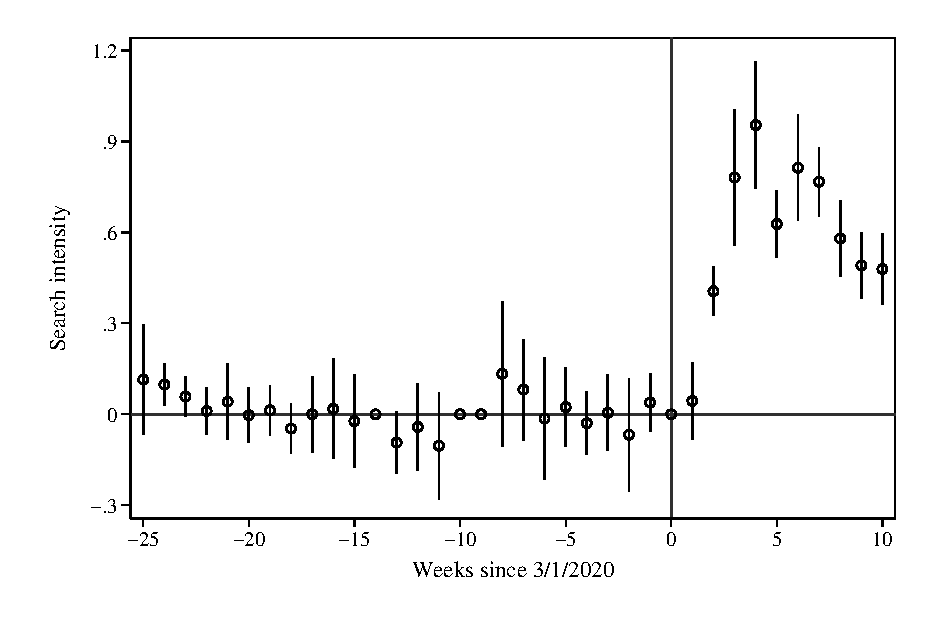
\includegraphics[width=\linewidth]{input/intensity_bh_replication_event_study_specific1.eps}
    \end{subfigure}%
    ~
    \begin{subfigure}[t]{0.45\textwidth}
    \caption{Parent-centered}
        \centering
        \includegraphics[width=\linewidth]{input/intensity_bh_replication_event_study_generic.eps}
    \end{subfigure}
    \caption{This widened the high-low SES search interest gap}
      \centering
      \begin{subfigure}[t]{0.45\textwidth}
      \caption{School-centered}
          \centering
          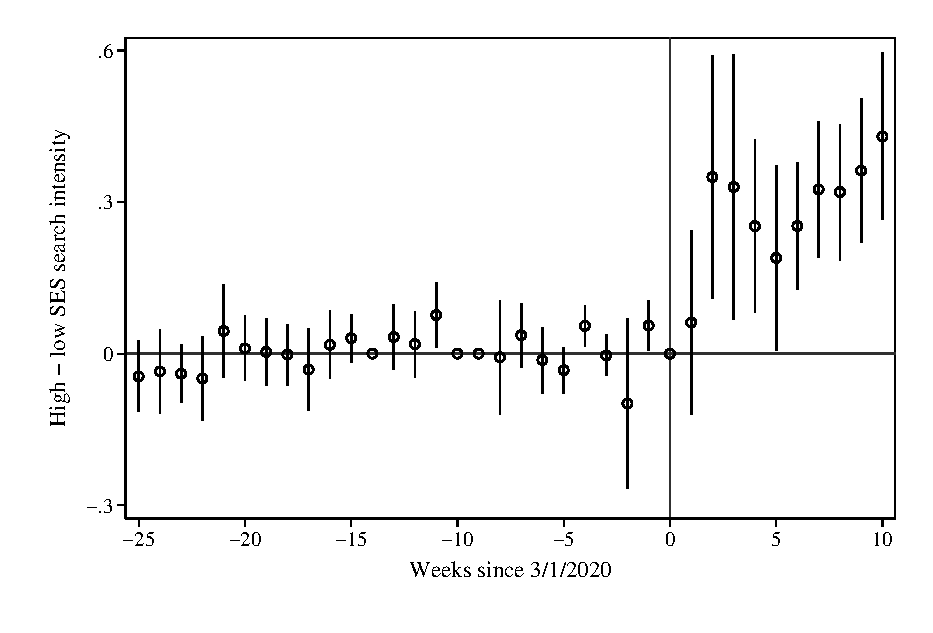
\includegraphics[width=\linewidth]{input/ses_bh_replication_event_study_specific1.eps}
      \end{subfigure}%
      ~
      \begin{subfigure}[t]{0.45\textwidth}
      \caption{Parent-centered}
          \centering
          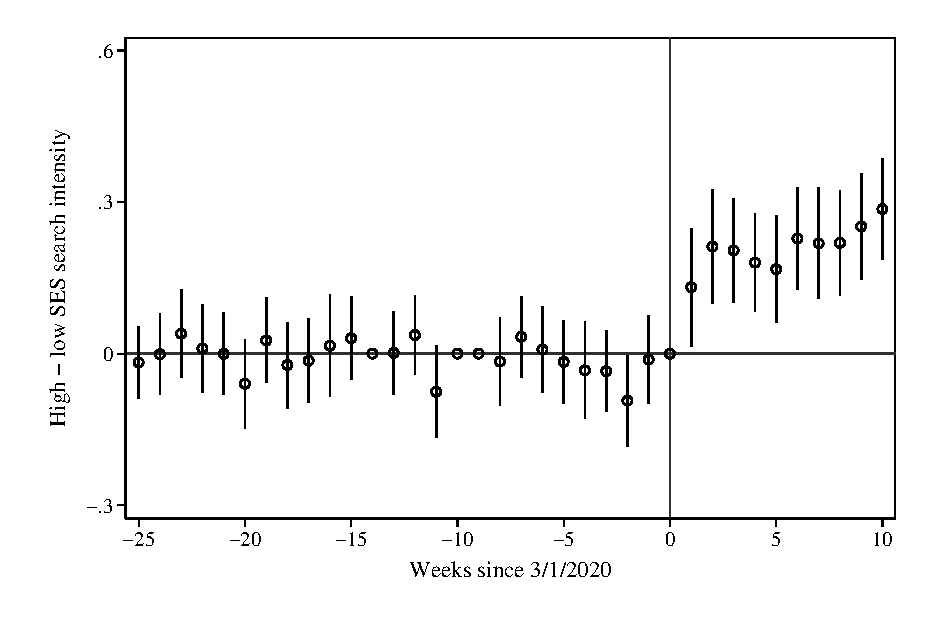
\includegraphics[width=\linewidth]{input/ses_bh_replication_event_study_generic.eps}
      \end{subfigure}
\begin{minipage}{\linewidth}
\footnotesize    \textit{Note:} This replicates DMA-level regressions from \cite{bh1}. I employ similar methodology in \ref{fig:eventstudy} and related appendix figures from the county-level. Panels (a) and (b) regress search interest on an indicator for relative week since March 1, 2020. Panels (c) and (d) are event studies by high-low SES group, defined by above or below median. SES is determined by taking the first principal component of income, broadband internet access, and presence of computer. All regressions include school year and week of year fixed effects. Intervals are 95\% confidence intervals and standard errors are clustered by state.
\end{minipage}
\end{figure}

\input{input/bh_replication_event_study_table_zero_one.tex}
\begin{table}[htbp] \centering
\def\sym#1{\ifmmode^{#1}\else\(^{#1}\)\fi}
\caption{\cite{bh1} Replication: Changes in Search Intensity, excluding low search intensity observations}
\scalebox{0.8}{
\begin{tabular*}{1\textwidth}{@{\extracolsep{\fill}}l*{4}{c}}
\midrule
&School-       &Parent-        &                       &               \\
&centered      &centered       &Google         &Khan   \\
&resources     &resources      &Classroom      &Academy\\
&(1)&(2)&(3)&(4)\\
\midrule
(A) Nationwide \\
\cmidrule{1-1}
Post COVID        &        0.52\sym{***}&        0.35\sym{***}&        0.76\sym{***}&        0.41\sym{***}\\
                    &      (0.05)         &      (0.02)         &      (0.05)         &      (0.03)         \\
\cmidrule{1-1}
(B) By median SES\\
\cmidrule{1-1}
Post COVID $\times$ Low-SES&        0.30\sym{***}&        0.21\sym{***}&        0.59\sym{***}&        0.30\sym{***}\\
                    &      (0.05)         &      (0.02)         &      (0.07)         &      (0.03)         \\
High SES            &       -0.04         &       -0.12\sym{***}&        0.07         &        0.01         \\
                    &      (0.06)         &      (0.03)         &      (0.10)         &      (0.06)         \\
Post COVID $\times$ High-SES&        0.44\sym{***}&        0.27\sym{***}&        0.35\sym{***}&        0.21\sym{***}\\
                    &      (0.10)         &      (0.03)         &      (0.11)         &      (0.05)         \\
                    &                     &                     &                     &                     \\
\cmidrule{1-1}
(C) By income, online access, race\\
\cmidrule{1-1}
Post COVID $\times$ HH mean income&        0.15\sym{***}&        0.09\sym{***}&        0.13\sym{***}&        0.08\sym{***}\\
                    &      (0.03)         &      (0.01)         &      (0.03)         &      (0.02)         \\
                    &                     &                     &                     &                     \\
Post COVID $\times$ \% of HH w/ broadband&        0.43\sym{***}&        0.34\sym{***}&        0.36\sym{***}&        0.30\sym{***}\\
                    &      (0.08)         &      (0.03)         &      (0.09)         &      (0.05)         \\
                    &                     &                     &                     &                     \\
Post COVID $\times$ \% of HH w/ computer&        0.54\sym{***}&        0.46\sym{***}&        0.47\sym{***}&        0.38\sym{***}\\
                    &      (0.10)         &      (0.04)         &      (0.10)         &      (0.07)         \\
                    &                     &                     &                     &                     \\
Post COVID $\times$ \% of schools in rural area&       -0.18\sym{***}&       -0.10\sym{***}&       -0.19\sym{***}&       -0.10\sym{***}\\
                    &      (0.03)         &      (0.01)         &      (0.03)         &      (0.02)         \\
                    &                     &                     &                     &                     \\
Post COVID $\times$ \% of students Black&       -0.09\sym{***}&       -0.04\sym{***}&       -0.02         &       -0.06\sym{***}\\
                    &      (0.03)         &      (0.02)         &      (0.04)         &      (0.02)         \\
                    &                     &                     &                     &                     \\
\hline
& 45845 & 40829 & 45682 & 44240
\end{tabular*}
}
\begin{minipage}{\textwidth}
\footnotesize    \textit{Note:} This replicates DMA-level regressions from \cite{bh1}. The outcomes are in log Google Trends search interest, where (1) and (2) are groupings of terms and (3) and (4) are specific terms. Post-COVID is after March 1, 2020. Panel (A) reveals that COVID-19 is a shock to search interest for resources. Panel (B) shows the results is a difference in differences regression on high-low SES, defined by the median. Panel (C) regresses on each of the individual factors that contribute to SES.
\end{minipage}
\end{table}


\begin{figure}[hbt!]
  \caption{Student online-learning engagement decreased by less in high-income counties after COVID-19}
    \centering
    \includegraphics[width=0.6\linewidth]{input/timetrend_engagement.eps}
    \begin{minipage}{\textwidth}
        \footnotesize
        \textit{Note:} This figure shows the trend in mean county-level standardized Zearn engagement
        split by quintile, with the middle three quintiles grouped.
        I drop the weeks containing Thanksgiving, Christmas, and New Years,
        as they are outliers.
    \end{minipage}
\end{figure}
\fi

\else
\clearpage
\begin{center} \Large \textbf{Appendix -- For Online Publication} \end{center}
\section{Exhibits}

\begin{figure}[hbt!]
    \caption{Student online-learning engagement decreased by less for high-income counties after COVID-19}
    \centering
    \includegraphics[width=0.7\linewidth]{input/timetrend_engagement.eps}
\end{figure}

\begin{figure}[hbt!]
  \caption{Student online-learning achievement only increased in high-income counties after COVID-19}
    \centering
    \includegraphics[width=0.7\linewidth]{input/timetrend_badges.eps}
\end{figure}

\begin{figure}[hbt!]
  \caption{Search intensity increased at the onset of COVID-19}
    \centering
    \includegraphics[width=0.7\linewidth]{input/timetrend_gtrends.eps}
\end{figure}


\begin{figure}[hbt!]
  \caption{Google Trends search intensity for educational resources increased more for highly-teleworkable counties}
    \centering
    \begin{subfigure}[t]{0.49\textwidth}
    \caption{School-centered}
        \centering
        \includegraphics[width=\linewidth]{input/eventstudyplot_specific1_inctele.eps}
    \end{subfigure}%
    ~
    \begin{subfigure}[t]{0.49\textwidth}
    \caption{Parent-centered}
        \centering
        \includegraphics[width=\linewidth]{input/eventstudyplot_generic_inctele.eps}
    \end{subfigure}
\end{figure}

\begin{figure}[hbt!]
  \caption{Teleworkability and income are highly, but not perfectly correlated}
    \centering
    \includegraphics[width=0.7\linewidth]{input/scatter_lninc_lntele.eps}
\end{figure}

\begin{figure}[hbt!]
  \caption{CBSA-level variation in teleworkability shows slight variation with income}
    \centering
    \begin{subfigure}[t]{0.65\textwidth}
    \caption{Log teleworkability}
        \centering
        \includegraphics[width=\linewidth]{input/map_lntele.eps}
    \end{subfigure}%

    \begin{subfigure}[t]{0.65\textwidth}
    \caption{Log median household income}
        \centering
        \includegraphics[width=\linewidth]{input/map_lninc.eps}
    \end{subfigure}
\end{figure}

\clearpage

\begin{table}[hbtp!]
  \centering
  \begin{tabular}{l c c c c c}
    \toprule
    \input{input/eventstudytable_mtitles.tex} \\
    \midrule
    (A) Post-COVID \\
    \midrule
    \input{input/eventstudytable_wks.tex} \\
    \midrule
    (B) Income Alone \\
    \midrule
    \input{input/eventstudytable_inc.tex} \\
    \midrule
    (C) Teleworkability Alone \\
    \midrule
    \input{input/eventstudytable_tele.tex} \\
    \midrule
    (D) Income + Teleworkability \\
    \midrule
    \input{input/eventstudytable_inctele.tex} \\
    \midrule
    \input{input/eventstudytable_beta.tex} \\
    \midrule
    \input{input/eventstudytable_N.tex} \\
    \bottomrule
  \end{tabular}
\end{table}

\if0
\begin{figure}[hbt!]
    \centering
    \caption{Student online-learning engagement decreased by less for high-income counties after COVID-19}
    \includegraphics[width=0.6\linewidth]{input/timetrend_engagement.eps}
\end{figure}

\begin{figure}[hbt!]
    \caption{COVID-19 was a shock to student and parent behavior with respect to education}
    \centering
    \begin{subfigure}[t]{0.4\textwidth}
    \caption{School-centered resources}
        \centering
        \includegraphics[width=\linewidth]{input/eventstudyplot_specific1_wks.eps}
    \end{subfigure}%
    ~
    \begin{subfigure}[t]{0.4\textwidth}
    \caption{Parent-centered resources}
        \centering
        \includegraphics[width=\linewidth]{input/eventstudyplot_generic_wks.eps}
    \end{subfigure}

    \begin{subfigure}[t]{0.4\textwidth}
    \caption{Student engagement}
        \centering
        \includegraphics[width=\linewidth]{input/eventstudyplot_engagement_wks.eps}
    \end{subfigure}%
    ~
    \begin{subfigure}[t]{0.4\textwidth}
    \caption{Student achievement}
        \centering
        \includegraphics[width=\linewidth]{input/eventstudyplot_badges_wks.eps}
    \end{subfigure}
\end{figure}

\begin{figure}[hbt!]
    \caption{Income inequalities in both parent and student behavior emerged at the onset of the pandemic}
    \centering
    \begin{subfigure}[t]{0.49\textwidth}
    \caption{School-centered resources}
        \centering
        \includegraphics[width=\linewidth]{input/eventstudyplot_specific1_inc.eps}
    \end{subfigure}%
    ~
    \begin{subfigure}[t]{0.49\textwidth}
    \caption{Parent-centered resources}
        \centering
        \includegraphics[width=\linewidth]{input/eventstudyplot_generic_inc.eps}
    \end{subfigure}

    \begin{subfigure}[t]{0.49\textwidth}
    \caption{Student engagement}
        \centering
        \includegraphics[width=\linewidth]{input/eventstudyplot_engagement_inc.eps}
    \end{subfigure}%
    ~
    \begin{subfigure}[t]{0.49\textwidth}
    \caption{Student achievement}
        \centering
        \includegraphics[width=\linewidth]{input/eventstudyplot_badges_inc.eps}
    \end{subfigure}
\end{figure}


\begin{figure}[hbt!]
    \caption{Highly teleworkable areas exhibit the same inequality as high income areas}
    \centering
    \begin{subfigure}[t]{0.49\textwidth}
    \caption{School-centered resources}
        \centering
        \includegraphics[width=\linewidth]{input/eventstudyplot_specific1_tele.eps}
    \end{subfigure}%
    ~
    \begin{subfigure}[t]{0.49\textwidth}
    \caption{Parent-centered resources}
        \centering
        \includegraphics[width=\linewidth]{input/eventstudyplot_generic_tele.eps}
    \end{subfigure}

    \begin{subfigure}[t]{0.49\textwidth}
    \caption{Student engagement}
        \centering
        \includegraphics[width=\linewidth]{input/eventstudyplot_engagement_tele.eps}
    \end{subfigure}%
    ~
    \begin{subfigure}[t]{0.49\textwidth}
    \caption{Student achievement}
        \centering
        \includegraphics[width=\linewidth]{input/eventstudyplot_badges_tele.eps}
    \end{subfigure}
\end{figure}
\fi
\begin{table}[hbtp!]
    \caption{Placebo robustness check: share of households with a computer}
    \label{tab:placebo_computer}
  \centering
  \scalebox{0.99}{
  \begin{tabular}{l c c c c c}
    \toprule
    \input{input/eventstudytable_mtitles.tex} \\
    \midrule
    (A) Post-COVID \\
    \midrule
    \input{input/eventstudytable_wks.tex} \\
    \midrule
    (B) Income Alone \\
    \midrule
    \input{input/eventstudytable_inc.tex} \\
    \midrule
    (C) Computer Alone \\
    \midrule
    \input{input/eventstudytable_comp.tex} \\
    \midrule
    (D) Income + Computer \\
    \midrule
    \input{input/eventstudytable_comptele.tex} \\
    \midrule
    \input{input/eventstudytable_betacomp.tex} \\
    \midrule
    \input{input/eventstudytable_N.tex} \\
    \bottomrule \\
  \end{tabular}
    }
  \begin{minipage}{\textwidth}
      \footnotesize
      \textit{Note}: This table displays the results of eight county level difference-in-differences regressions on the following dependent variables: (1) the natural log of Google Trends search interest for school-centered resources; (2) the natural log of Google Trends search interest parent-centered resources;  (3) Zearn engagement normalized relative to a base period from January 6-February 7,  2020; and (4) Zearn badges normalized relative to a base period from January 6-February 7,  2020. All regression include fixed effects for year and week of year.
      Panel A reveals the first-order effect of COVID-19 on the outcomes.
      Panel B is a difference-in-differences on log income.
      Panel C is a difference-in-differences on the log share of households with a computer.
      Panel D includes both sets of interaction terms.
      I include full interactions, despite not displaying the coefficients on log income and log computer share.
      Note from Eq. \refeq{inctele} that $\gamma$ is the coefficient on Post COVID $\times$ Income, so
      $100 \times \frac{\gamma_B-\gamma_D}{\gamma_B}$ is the percentage change in this coefficient
      when log computer share is included.
      I drop Thanksgiving, Christmas, and New Years, as these are outliers, but the results do not change significantly when they are included.
      I also drop the first three weeks of March, as schools were actively closing during this time.
      Standard errors are in parentheses and clustered by state.
  \end{minipage}


\end{table}

\begin{table}[hbtp!]
    \caption{Placebo robustness check: share of households with a broadband internet connection}
    \label{tab:placebo_internet}
  \centering
  \begin{tabular}{l c c c c c}
    \toprule
    \input{input/eventstudytable_mtitles.tex} \\
    \midrule
    (A) Post-COVID \\
    \midrule
    \input{input/eventstudytable_wks.tex} \\
    \midrule
    (B) Income Alone \\
    \midrule
    \input{input/eventstudytable_inc.tex} \\
    \midrule
    (C) Computer Alone \\
    \midrule
    \input{input/eventstudytable_broad.tex} \\
    \midrule
    (D) Income + Computer \\
    \midrule
    \input{input/eventstudytable_broadtele.tex} \\
    \midrule
    \input{input/eventstudytable_betabroad.tex} \\
    \midrule
    \input{input/eventstudytable_N.tex} \\
    \bottomrule \\
  \end{tabular}
  \begin{minipage}{\textwidth}
      \footnotesize
      \textit{Note}: This table displays the results of eight county level difference-in-differences regressions on the following dependent variables: (1) the natural log of Google Trends search interest for school-centered resources; (2) the natural log of Google Trends search interest parent-centered resources;  (3) Zearn engagement normalized relative to a base period from January 6-February 7,  2020; and (4) Zearn badges normalized relative to a base period from January 6-February 7,  2020. All regression include fixed effects for year and week of year.
      Panel A reveals the first-order effect of COVID-19 on the outcomes.
      Panel B is a difference-in-differences on log income.
      Panel C is a difference-in-differences on the log share of households with broadband internet.
      Panel D includes both sets of interaction terms.
      I include full interactions, despite not displaying the coefficients on log income and log internet.
      Note from Eq. \refeq{inctele} that $\gamma$ is the coefficient on Post COVID $\times$ Income, so
      $100 \times \frac{\gamma_B-\gamma_D}{\gamma_B}$ is the percentage change in this coefficient
      when internet is included.
      I drop Thanksgiving, Christmas, and New Years, as these are outliers, but the results do not change significantly when they are included.
      I also drop the first three weeks of March, as schools were actively closing during this time.
      Standard errors are in parentheses and clustered by state.
  \end{minipage}


\end{table}

\if0
\begin{figure}[hbt!]
    \centering
    \begin{subfigure}[t]{0.65\textwidth}
    \caption{Parent-centered resources}
        \centering
        \includegraphics[width=\linewidth]{input/map_generic.eps}
    \end{subfigure}%

    \begin{subfigure}[t]{0.65\textwidth}
    \caption{School-centered resources}
        \centering
        \includegraphics[width=\linewidth]{input/map_specific1.eps}
    \end{subfigure}
\end{figure}


\begin{figure}[hbt!]
    \centering
    \begin{subfigure}[t]{0.65\textwidth}
    \caption{Zearn engagement}
        \centering
        \includegraphics[width=\linewidth]{input/map_engagement.eps}
    \end{subfigure}%

    \begin{subfigure}[t]{0.65\textwidth}
    \caption{Zearn badges}
        \centering
        \includegraphics[width=\linewidth]{input/map_badges.eps}
    \end{subfigure}
\end{figure}

\begin{figure}[hbt!]
    \centering
    \begin{subfigure}[t]{0.65\textwidth}
    \caption{Share of households with broadband internet}
        \centering
        \includegraphics[width=\linewidth]{input/map_broad.eps}
    \end{subfigure}%

    \begin{subfigure}[t]{0.65\textwidth}
    \caption{Share of households with computer}
        \centering
        \includegraphics[width=\linewidth]{input/map_comp.eps}
    \end{subfigure}
\end{figure}

\begin{figure}[hbt!]
    \centering
    \begin{subfigure}[t]{0.65\textwidth}
    \caption{Teleworkability share}
        \centering
        \includegraphics[width=\linewidth]{input/map_tele.eps}
    \end{subfigure}%

    \begin{subfigure}[t]{0.65\textwidth}
    \caption{Work from home score}
        \centering
        \includegraphics[width=\linewidth]{input/map_wfhscore.eps}
    \end{subfigure}
\end{figure}

\begin{figure}[hbt!]
    \centering
    \begin{subfigure}[t]{0.75\textwidth}
    \caption{Student achievement}
        \centering
        \includegraphics[width=\linewidth]{input/eventstudyplot_badges_inccomp_long.eps}
    \end{subfigure}%
\end{figure}

\begin{figure}[hbt!]
    \centering
    \begin{subfigure}[t]{0.75\textwidth}
    \caption{Student achievement}
        \centering
        \includegraphics[width=\linewidth]{input/eventstudyplot_badges_incbroad_long.eps}
    \end{subfigure}%
\end{figure}
\fi

\if0
\begin{figure}[hbt!]
    \caption{\cite{bh1} Replication: COVID-19 is a shock search interest}
    \centering
    \begin{subfigure}[t]{0.45\textwidth}
    \caption{School-centered}
        \centering
        \includegraphics[width=\linewidth]{input/intensity_bh_replication_event_study_specific1.eps}
    \end{subfigure}%
    ~
    \begin{subfigure}[t]{0.45\textwidth}
    \caption{Parent-centered}
        \centering
        \includegraphics[width=\linewidth]{input/intensity_bh_replication_event_study_generic.eps}
    \end{subfigure}
    \caption{This widened the high-low SES search interest gap}
      \centering
      \begin{subfigure}[t]{0.45\textwidth}
      \caption{School-centered}
          \centering
          \includegraphics[width=\linewidth]{input/ses_bh_replication_event_study_specific1.eps}
      \end{subfigure}%
      ~
      \begin{subfigure}[t]{0.45\textwidth}
      \caption{Parent-centered}
          \centering
          \includegraphics[width=\linewidth]{input/ses_bh_replication_event_study_generic.eps}
      \end{subfigure}
\begin{minipage}{\linewidth}
\footnotesize    \textit{Note:} This replicates DMA-level regressions from \cite{bh1}. I employ similar methodology in \ref{fig:eventstudy} and related appendix figures from the county-level. Panels (a) and (b) regress search interest on an indicator for relative week since March 1, 2020. Panels (c) and (d) are event studies by high-low SES group, defined by above or below median. SES is determined by taking the first principal component of income, broadband internet access, and presence of computer. All regressions include school year and week of year fixed effects. Intervals are 95\% confidence intervals and standard errors are clustered by state.
\end{minipage}
\end{figure}

\input{input/bh_replication_event_study_table_zero_one.tex}
\begin{table}[htbp] \centering
\def\sym#1{\ifmmode^{#1}\else\(^{#1}\)\fi}
\caption{\cite{bh1} Replication: Changes in Search Intensity, excluding low search intensity observations}
\scalebox{0.8}{
\begin{tabular*}{1\textwidth}{@{\extracolsep{\fill}}l*{4}{c}}
\midrule
&School-       &Parent-        &                       &               \\
&centered      &centered       &Google         &Khan   \\
&resources     &resources      &Classroom      &Academy\\
&(1)&(2)&(3)&(4)\\
\midrule
(A) Nationwide \\
\cmidrule{1-1}
Post COVID        &        0.52\sym{***}&        0.35\sym{***}&        0.76\sym{***}&        0.41\sym{***}\\
                    &      (0.05)         &      (0.02)         &      (0.05)         &      (0.03)         \\
\cmidrule{1-1}
(B) By median SES\\
\cmidrule{1-1}
Post COVID $\times$ Low-SES&        0.30\sym{***}&        0.21\sym{***}&        0.59\sym{***}&        0.30\sym{***}\\
                    &      (0.05)         &      (0.02)         &      (0.07)         &      (0.03)         \\
High SES            &       -0.04         &       -0.12\sym{***}&        0.07         &        0.01         \\
                    &      (0.06)         &      (0.03)         &      (0.10)         &      (0.06)         \\
Post COVID $\times$ High-SES&        0.44\sym{***}&        0.27\sym{***}&        0.35\sym{***}&        0.21\sym{***}\\
                    &      (0.10)         &      (0.03)         &      (0.11)         &      (0.05)         \\
                    &                     &                     &                     &                     \\
\cmidrule{1-1}
(C) By income, online access, race\\
\cmidrule{1-1}
Post COVID $\times$ HH mean income&        0.15\sym{***}&        0.09\sym{***}&        0.13\sym{***}&        0.08\sym{***}\\
                    &      (0.03)         &      (0.01)         &      (0.03)         &      (0.02)         \\
                    &                     &                     &                     &                     \\
Post COVID $\times$ \% of HH w/ broadband&        0.43\sym{***}&        0.34\sym{***}&        0.36\sym{***}&        0.30\sym{***}\\
                    &      (0.08)         &      (0.03)         &      (0.09)         &      (0.05)         \\
                    &                     &                     &                     &                     \\
Post COVID $\times$ \% of HH w/ computer&        0.54\sym{***}&        0.46\sym{***}&        0.47\sym{***}&        0.38\sym{***}\\
                    &      (0.10)         &      (0.04)         &      (0.10)         &      (0.07)         \\
                    &                     &                     &                     &                     \\
Post COVID $\times$ \% of schools in rural area&       -0.18\sym{***}&       -0.10\sym{***}&       -0.19\sym{***}&       -0.10\sym{***}\\
                    &      (0.03)         &      (0.01)         &      (0.03)         &      (0.02)         \\
                    &                     &                     &                     &                     \\
Post COVID $\times$ \% of students Black&       -0.09\sym{***}&       -0.04\sym{***}&       -0.02         &       -0.06\sym{***}\\
                    &      (0.03)         &      (0.02)         &      (0.04)         &      (0.02)         \\
                    &                     &                     &                     &                     \\
\hline
& 45845 & 40829 & 45682 & 44240
\end{tabular*}
}
\begin{minipage}{\textwidth}
\footnotesize    \textit{Note:} This replicates DMA-level regressions from \cite{bh1}. The outcomes are in log Google Trends search interest, where (1) and (2) are groupings of terms and (3) and (4) are specific terms. Post-COVID is after March 1, 2020. Panel (A) reveals that COVID-19 is a shock to search interest for resources. Panel (B) shows the results is a difference in differences regression on high-low SES, defined by the median. Panel (C) regresses on each of the individual factors that contribute to SES.
\end{minipage}
\end{table}


\begin{figure}[hbt!]
  \caption{Student online-learning engagement decreased by less in high-income counties after COVID-19}
    \centering
    \includegraphics[width=0.6\linewidth]{input/timetrend_engagement.eps}
    \begin{minipage}{\textwidth}
        \footnotesize
        \textit{Note:} This figure shows the trend in mean county-level standardized Zearn engagement
        split by quintile, with the middle three quintiles grouped.
        I drop the weeks containing Thanksgiving, Christmas, and New Years,
        as they are outliers.
    \end{minipage}
\end{figure}
\fi


\textit{Note: Appendix omitted to meet the page requirements. Link to full paper on the first page.}
\fi

\end{document}
